\section{Системы контроля версий}
\subsection{Что такое контроль версий, и зачем он вам нужен?}

\begin{frame}[t]{Что такое контроль версий, и зачем он вам нужен?}

Система контроля версий (СКВ) — это система, регистрирующая изменения в одном или нескольких файлах с тем, 
чтобы в дальнейшем была возможность вернуться к определённым старым версиям этих файлов. 

СКВ даёт возможность возвращать отдельные файлы к прежнему виду, 
возвращать к прежнему состоянию весь проект, 
просматривать происходящие со временем изменения, определять, 
кто последним вносил изменения во внезапно переставший работать модуль, 
кто и когда внёс в код какую-то ошибку, и многое другое. 
Вообще, если, пользуясь СКВ, вы всё испортите или потеряете файлы, всё можно будет легко восстановить. 

Системы контроля версий:
\begin{itemize}
  \item Централизованные 
  \item Децентрализованные
\end{itemize}

\end{frame}

\subsection{Системы контроля версий: локальные, централизованные, распределённые}

\begin{frame}[t]{Subversion}

Бесплатная система управления версиями с открытым исходным кодом.
Subversion позволяет управлять файлами и каталогами, а так же сделанными в них изменениями
во времени. Это позволяет восстановить более ранние версии данных, даѐт возможность изучить
историю всех изменений. Благодаря этому многие считают систему управления версиями своего
рода «машиной времени».

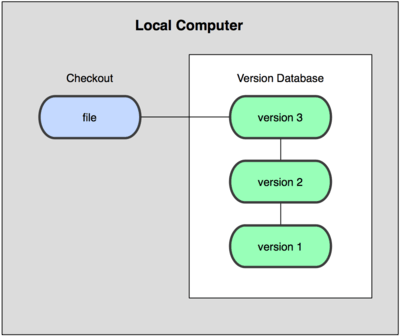
\includegraphics[width=0.5\textwidth]{git/rcs.png}

\end{frame}

\begin{frame}[t]{Централизованные системы контроля версий}
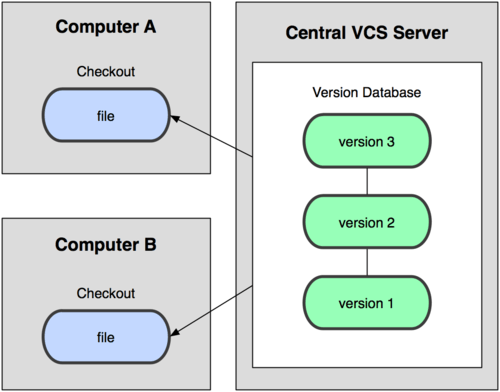
\includegraphics[width=0.5\textwidth]{git/central.png}
\end{frame}

\begin{frame}[t]{Распределённые системы контроля версий}
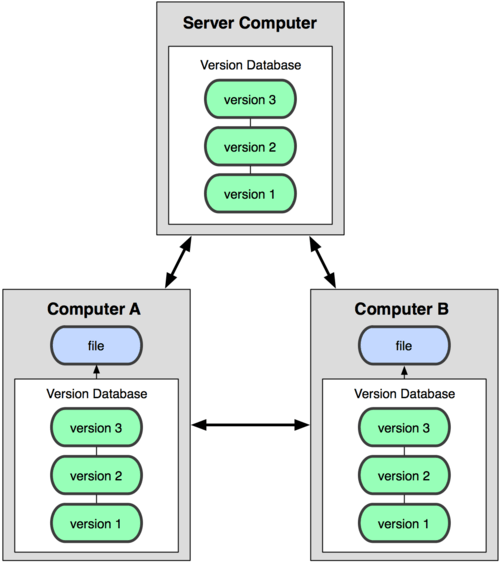
\includegraphics[width=0.5\textwidth]{git/distrib.png}
\end{frame}

\begin{frame}[t]{Git}

Распределённая система управления версиями. 
Проект был создан Линусом Торвальдсом для управления разработкой ядра Linux, первая версия выпущена 7 апреля 2005 года. 
На сегодняшний день его поддерживает Джунио Хамано.

Примерами проектов, использующих Git, являются:
ядро Linux, Android, Drupal, Cairo, GNU Core Utilities, Mesa, Wine, Chromium, Compiz Fusion, FlightGear, jQuery, PHP, NASM, MediaWiki, DokuWiki, Qt и некоторые дистрибутивы Linux 

\url{}

\end{frame}

\begin{frame}[t]{Откуда скачать и установить Git?}


Для Windows --- \url{https://git-for-windows.github.io}

Нажимаете \textbf{Download}, скачивается исполняемый файл, например 
\textbf{Git-2.6.1-64-bit.exe}

Устанавливаете его. 

После установки должна появится в командной строке команда:
\texttt{git}

\end{frame}

 
\subsection{История версий, ветки}
\begin{frame}[t]{Основные команды Git}

\texttt{git init} --- создание нового git-репозитория в текущей папке.
С этого момента в этой папке появляется <<машина времени>> для изменений.
Если вы сделали изменение и зафиксировали его, вы всегда можете откатиться к этой версии.

При успешной инициализации выводится сообщение:
Initialized empty Git repository in FolderName

\texttt{git add} --- добавление файлов в систему контроля версий.
Например: \texttt{git add a.cpp} --- добавить файл a.cpp в СКВ.
\texttt{git add *.cpp} --- добавить все .cpp файлы в СКВ. 
\texttt{git add .} --- добавить все файлы и все каталоги с подкаталогами в СКВ. 

\end{frame}

\subsection{Почитать про Git}
\begin{frame}[t]{Основные команды Git}

\end{frame}
                                         